%%% Kapitola – Výzvy a problémy
%%%%% Wording: ✅
%%%%% Styling: ✅
%%%%% References: ✅
%%%%% Grammar: ✅
%%% --------------------------------------------------------------
\chapter{Výzvy a problémy}
\label{ch:vyzvy-a-problemy}
Tato kapitola se zabývá zajímavými výzvami a problémy, které se vyskytly během vývoje aplikace a které stojí za zmínku.
Každá sekce popisuje konkrétní problém, který byl řešen, různé alternativy, které byly zvažovány, a konečná řešení, která byla implementována.
Sdílením těchto zkušeností lze dosáhnout hlubšího porozumění vývojového procesu a složitého rozhodování, které je zapotřebí při vývoji komplexních aplikací.

%%% Sekce – Vykreslování interaktivního plánu sezení pomocí SVG
%%%%% Wording: ✅
%%%%% Styling: ✅
%%%%% References: ✅
%%%%% Grammar: ✅
%%% --------------------------------------------------------------


\section{Vykreslování interaktivního plánu sezení pomocí SVG}
\label{sec:vyzvy-a-problemy-rendering-sedadel}
Vykreslování interaktivního plánu sezení představovalo počáteční výzvu, což bylo především způsobeno složitostí a dynamickou povahou virtuálních map.
Byly zvažovány různé technologie, jako je inline \ac{svg}, \foreign{Canvas API}\footnote{\foreign{Canvas API} je \ac{api} pro vykreslování 2D grafiky a animací pomocí JavaScriptu a je součástí HTML5 specifikace\cite{mdn_api_canvas_api}.} a \foreign{Three.js}\footnote{\foreign{Three.js} je knihovna pro JavaScript, která umožňuje vytvářet a vykreslovat 3D grafiku v prohlížeči\cite{mdn_games_techniques_3d_on_the_web_building_up_a_basic_demo_with_three_js}.}.

Po důkladném zvážení byla vybrána technologie inline \ac{svg}, jelikož poskytovala největší flexibilitu, nezávislost na externích knihovnách a nejjednodušší implementaci\cite{s_blog_seating_plan_rendering}.
Tato metoda umožnila jednoduché a přímočaré interakce s \ac{dom}, což usnadnilo vývoj interaktivní mapy sedadel.

Nicméně animace a transformace \ac{svg} představovaly další problém.
\ac{svg} a \ac{html} prvky se chovají odlišně, pokud jde o jejich počáteční body neboli tzv. \foreign{origin points}, jak je znázorněno na obrázku~\ref{fig:css-tricks-svg-transforms} níže.

\begin{figure}[H]
    \centering
    \caption{Počáteční body SVG a HTML}
    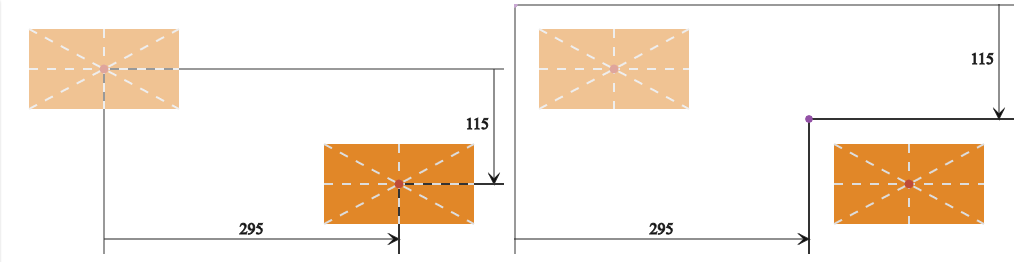
\includegraphics[width=\textwidth]{\FIGDIR/css-tricks-svg-transforms}
    \source[\citeauthor{ct_css_tricks_com_transforms_on_svg_elements}]{}
    \label{fig:css-tricks-svg-transforms}
\end{figure}

To způsobilo neočekávané chování při implementaci určitých funkcionalit transformace prvků na mapě.
Tento problém byl nakonec vyřešení hlubším porozuměním transformacím \ac{svg} a jejich vztahu k \ac{html} prvkům.

%%% Sekce – Absence API a jeho simulace
%%%%% Wording: ✅
%%%%% Styling: ✅
%%%%% References: ✅
%%%%% Grammar: ✅
%%% --------------------------------------------------------------


\section{Absence API a jeho simulace}
\label{sec:vyzvy-a-problemy-absence-api}
Vývoj aplikace probíhal v nepřítomnosti dedikovaného \ac{api}.
To znamenalo, že bylo zapotřebí definovat datové struktury a simulovat různá \ac{api} volání v rámci kódu.
Toho bylo docíleno implementací asynchronních funkcí s umělým zpožděním, které napodobovaly skutečná \ac{api} volání.

Takové řešení poskytovalo požadovanou funkcionalitu, ale přinášelo také výzvu zajištění konzistence dat a správy potenciálních chyb, podobně jako by se očekávalo u skutečných \ac{api} volání.
Tato výzva byla vyřešena jednak vytvořením vlastního mock \ac{api} endpointu díky Next.js \ac{api} routingu\cite{n_basics_api_routes} a jednak vytvořením \ac{api} klienta, který poskytoval konzistentní rozhraní pro potenciální komunikaci se skutečným \ac{api}.

%%% Sekce – Zachování jednoduchosti v komplexní aplikaci
%%%%% Wording: ✅
%%%%% Styling: ✅
%%%%% References: ✅
%%%%% Grammar: ✅
%%% --------------------------------------------------------------


\section{Zachování jednoduchosti v komplexní aplikaci}
\label{sec:vyzvy-a-problemy-zachovani-jednoduchosti}
Jednou z opakujících se výzev během vývoje byl vnitřní osobní konflikt při konstrukci komplexní aplikace produkční kvality, která by zároveň zachovávala jednoduchost a přímočarost.
Například implementace komplexního routingu a správy stavu byla zvažována, ale nakonec byla zavrhnuta ve prospěch jednoduchého řešení, které bylo dostatečné pro potřeby aplikace.

K tomuto řešení byla například implementována vlastního komponenta \texttt{MultiView}, která podmíněně vykresluje zadané pohledy na základě jednoho aktivního, čímž se obešla potřeba složitého routování.
Tato strategie zachovala jednoduchost aplikace, aniž by to mělo vliv na její funkčnost.

Dalším problémem bylo rozhodování, které funkcionality pro produkční nasazení implementovat; funkcionality jako je internacionalizace, přístupnost, optimalizace pro vyhledávače – \ac{seo}, správa uživatelských relací či aktualizace dat v reálném čase pomocí \ac{ws}\cite{mdn_api_websockets_api}.
Nakonec bylo rozhodnuto zaměřit se na základní funkčnost aplikace a implementaci těchto funkcí ponechat na možné budoucí iterace.

%%% Sekce – Shrnutí
%%%%% Wording: ✅
%%%%% Styling: ✅
%%%%% References: ✅
%%%%% Grammar: ✅
%%% --------------------------------------------------------------


\section{Shrnutí}
\label{sec:vyzvy-a-problemy-shrnuti}
Tato kapitola zkoumala některé z kritických výzev, které se objevily během vývoje aplikace.
Od vykreslování interaktivní mapy pomocí \ac{svg}, simulace \ac{api} volání, až po zachování jednoduchosti v komplexní a rostoucí aplikaci.
Každá výzva přinesla své jedinečné problémy, učící příležitosti a zajímavá řešení, která ukázala složitý proces vývoje frontendových aplikací v praxi.
